\documentclass{article}
\usepackage[utf8]{inputenc}
\usepackage{tikz}
\usetikzlibrary{shapes,arrows}
\usepackage[ruled,vlined]{algorithm2e}
\usepackage{algpseudocode}
\usepackage{multicol}
\renewcommand{\contentsname}{{\Huge Table de Matières}}
\usepackage{titlesec}
\usepackage{xcolor}
\usepackage{listings}
\usepackage{graphicx}
\usepackage[normalem]{ulem}
\titleformat{\section}{\Huge\bfseries}{\thesection}{1em}{}
\titleformat{\subsection}{\huge\bfseries}{\thesubsection}{1em}{}
\titleformat{\subsubsection}{\LARGE\bfseries}{\thesubsubsection}{1em}{}
\begin{document}
\begin{center}
\pagenumbering{gobble}
\linespread{2.0}\selectfont

{\Huge U}{\huge NIVERSITÉ DE }{\Huge M}{\huge ONTPELLIER}\\
{\huge L3}{\LARGE ~INFORMATIQUE }
\\~\\~\\~\\~\\
{\Large\textbf{TOURNOI SPORTIF\\"ESport"}}
\\~\\~\\~\\~\\

\linespread{1}\selectfont

RAPPORT DE PROJET\\~\\
PROJET INFORMATIQUE COMMUN AVEC\\
 HLIN510 ET HLIN511\\
\vfill
\end{center}
\begin{multicols}{2}
\begin{flushleft}
\textbf{Etudiants:}\\
~~M. Benjamin Baska\\
~~M. Kevin Lastra
\end{flushleft}
\columnbreak
\begin{flushright}
\textbf{Enseignant responsable:}\\
M. Pierre Pompidor~~~\\
M. Michele Meynard~~\\
M. Pascale Poncelet~~~
\end{flushright}
\end{multicols}
\newpage
\tableofcontents
\newpage
{\textbf{\Huge Introduction}}\\~\\~\\
~~Notre groupe, composé de Benjamin Baska et Kevin Lastra, a travaillé sur le développement de la page Web "ESport" comme projet commun des modules HLIN510 et HLIN511.
\newpage
\section{Organisation du projet}
\subsection{Objectifs et cahier des charges}
Le projet consiste à développer un site de gestion de tournoi sportif de Jeux vidéo, où les organisateur pourrons créer et manipuler des tournois, et aux équipes de joueur de s’inscrire au tournois.\\~\\
Les objectives principal sont:
\begin{itemize}
\item Créer un page web fonctionnelle.
\item Créer un system de comptes pour les organisateur et les joueur.
\item Créer un system de gestion de tournois pour les organisateur.
\item Créer et manipuler une base de donnes mysql.
\end{itemize}
\subsection{Division du travaille}
\subsection{Outils de travaille}
\subsubsection{Langage de programmation}
Les Langages qu'on a utiliser dans le développement de cette page web sont:
\begin{itemize}
\item HTML
\item Javascript
\item PHP
\end{itemize}
\subsubsection{Éditeur de Texte}
La production du projet est réalisée grâce à plusieurs éditeur de text:
\begin{itemize}
\item Emacs
\item Visual Code
\end{itemize}
\subsubsection{Utils Web}
Dans le développement de la page web on a utiliser divers utiles:
\begin{itemize}
\item Framework: Bootstrap
\item Gestionnaire de Base de Donnes: PHPmyAdmin
\end{itemize}
\subsubsection{Travaille collaboratif}
Pour pouvoir maintenir une bonne gestion du projet collaboratif a distance, sur tout dans le condition actuel du confinement a cause du Covid-19, on a utiliser divers programme:
\begin{itemize}
\item GitHub
\item Discord
\end{itemize}
Aussi grâce a la création d'un serveur public Apache on pouvez accéder au projet via ssh et comme ça maintenir une version stable du projet.
\section{Conception}
\subsection{CLIENT}
\subsubsection{HTML}
\subsubsection{TypeScript} 
\subsubsection{Bootstrap}
\subsubsection{Angular}
\subsection{SERVEUR}
\subsubsection{Base de Donnes}
{\textbf{\Large Modelé Entité/Association}\\

\begin{figure}[h]
\centering
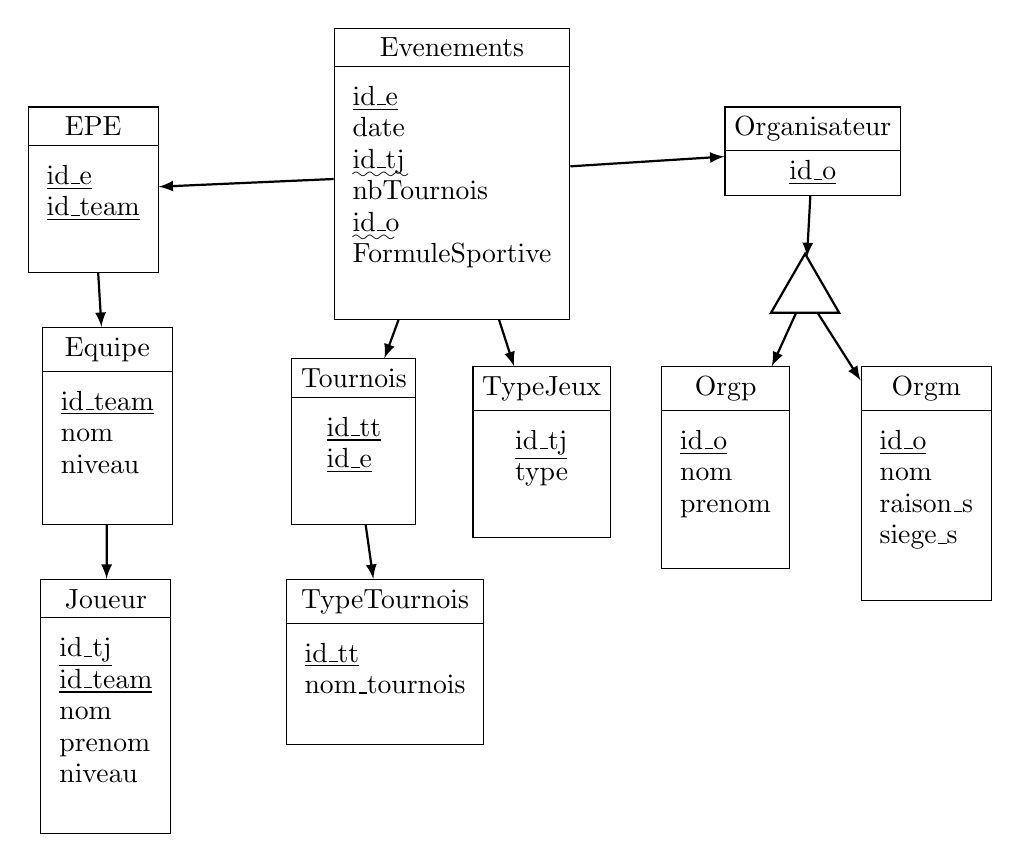
\begin{tikzpicture}[
					double/.style={draw, anchor=text, 		rectangle split, rectangle split parts=2},
					triple/.style={draw, anchor=text, rectangle split, rectangle split parts=3},
					triangle/.style={draw, shape=regular polygon, regular polygon sides=3,draw,thick,inner sep=0pt, minimum size=1cm, inner sep=-1.2cm, outer sep=0pt}]
					
    % Place nodes
    \node [double] (A) at (0,4){Evenements
    	\nodepart{second}
    	\tikz{
    	\node at (0,0) {\underline{id\_e}};
    	\node at (0,-0.4) {date};
    	\node at (0,-0.8) {\uwave{id\_tj}};
    	\node at (0,-1.2) {nbTournois};
    	\node at (0,-1.6) {\uwave{id\_o}};
    	\node at (0,-2) {FormuleSportive};
    }};
    \node [double] (B) at (-4,3){EPE
    	\nodepart{second}
    	\tikz{
    	\node at (0,0) {\underline{id\_e}};
    	\node at (0,-0.4) {\underline{id\_team}};
    }};
    \node [double] (C) at (-1,-0.2){Tournois
    	\nodepart{second}
    	\tikz{
    	\node at (0,0) {\underline{id\_tt}};
    	\node at (0,-0.4) {\underline{id\_e}};
    }};
	\node [double] (D) at (1.3,-0.3){TypeJeux
    	\nodepart{second}
    	\tikz{
    	\node at (0,0) {\underline{id\_tj}};
    	\node at (0,-0.4) {type};
    }};
    \node [double] (E) at (4.5,3){Organisateur
    	\nodepart{second}
    	{\underline{id\_o}}
    };
    \node [double] (F) at (-4,0.2){Equipe
    	\nodepart{second}
    	\tikz{
		\node at (0,0) {\underline{id\_team}};
    	\node at (0,-0.4) {nom};
    	\node at (0,-0.8) {niveau};    	
    }};
    \node [double] (G) at (-1,-3){TypeTournois
    	\nodepart{second}
    	\tikz{
		\node at (0,0) {\underline{id\_tt}};
    	\node at (0,-0.4) {nom\_tournois};	    	
    }};
    \node [double] (H) at (-4,-3){Joueur
    	\nodepart{second}
    	\tikz{
		\node at (0,0) {\underline{id\_tj}};
		\node at (0,-0.4) {\underline{id\_team}};
    	\node at (0,-0.8) {nom};	    	
    	\node at (0,-1.2) {prenom};	    
    	\node at (0,-1.6) {niveau};		
    }};
    \node [double] (I) at (4,-0.3){Orgp
    	\nodepart{second}
    	\tikz{
		\node at (0,0) {\underline{id\_o}};
		\node at (0,-0.4) {nom};
    	\node at (0,-0.8) {prenom};		
    }};
    \node [double] (J) at (6.5,-0.3){Orgm
    	\nodepart{second}
    	\tikz{
		\node at (0,0) {\underline{id\_o}};
		\node at (0,-0.4) {nom};
    	\node at (0,-0.8) {raison\_s};		
    	\node at (0,-1.2) {siege\_s};
    }};
    \node [triangle] (K) at (5.4, 1){};
    \draw[thick,-latex] (A) edge (B);
    \draw[thick,-latex] (A) edge (C);
    \draw[thick,-latex] (A) edge (D);
    \draw[thick,-latex] (A) edge (E);
	\draw[thick,-latex] (B) edge (F);	
	\draw[thick,-latex] (F) edge (H);
	\draw[thick,-latex] (C) edge (G);
	\draw[thick,-latex] (E) edge (K);
	\draw[thick,-latex] (K) edge (I);
    \draw[thick,-latex] (K) edge (J);	
    % Draw edges
    
\end{tikzpicture}~\\
\caption{Graphe du Modelé Entité/Association}

\end{figure}~\\
\newpage
{\textbf{\Large Modelé Relationnelle}\\

evenement(\underline{id\_e}, date, \uwave{id\_tj}, nb\_tournois, \uwave{id\_o}, formule\_sportive)

typejeux(\underline{id\_tj}, type)

tournois(\underline{id\_tt}, \underline{id\_e})

typetournois(\underline{id\_tt}, nom\_tournois)

EPE(\underline{id\_e}, \underline{id\_team})

equipe(\underline{id\_team}, nom, niveau)

joueur(\underline{id\_j}, \uwave{id\_team}, nom, prenom, niveau)

organisateur(\underline{id\_o} , ...)

org\_physique(\underline{id\_o}, nom, prenom)

org\_morale(\underline{id\_o}, nom, raison\_s, siege\_s)

\subsubsection{PHP}
\section{Résultat}
\subsection{La Page}
\subsection{CONCLUSION}
\section{Bibliographie}
\end{document}